\documentclass[11pt,a4paper]{article}

% ---------- arxiv-style preamble ----------
\usepackage[margin=1in]{geometry}
\usepackage{amsmath,amssymb,amsthm}
\usepackage{graphicx}
\usepackage{booktabs}
\usepackage{siunitx}
\DeclareSIUnit{\rydberg}{Ry}
\DeclareSIUnit{\atm}{atm}
\usepackage{hyperref}
\usepackage{xcolor}
\usepackage[numbers,sort&compress]{natbib}
\usepackage{tikz}
\usetikzlibrary{positioning,arrows.meta}
% pgfplots — shipped by default (the 58p monograph build had every agent add
% this by hand + `sudo tlmgr install pgfplots`). The fig02_line.tex standalone
% uses it; the compat line is pinned so axis behaviour is deterministic.
\usepackage{pgfplots}
\pgfplotsset{compat=1.18}
\usepackage{caption}
\usepackage{listings}
\usepackage{array}
\captionsetup{font=small,labelfont=bf}
\hypersetup{
  colorlinks=true,
  linkcolor=blue!50!black,
  citecolor=blue!50!black,
  urlcolor=blue!50!black
}

% ---------- tier badges (color-coded text labels; font-independent) ----------
% This BasicTeX install has no color-emoji font fallback, so the tier badges
% render as bracketed colored words. Each maps 1:1 to a hexa verify tier.
\newcommand{\tierBlue}{\textcolor{blue!60!black}{[\textsc{formal}]}}
\newcommand{\tierGreen}{\textcolor{teal}{[\textsc{green}]}}
\newcommand{\tierYellow}{\textcolor{olive}{[\textsc{cited}]}}
\newcommand{\tierOrange}{\textcolor{orange!85!black}{[\textsc{deferred}]}}
\newcommand{\tierRed}{\textcolor{red!75!black}{[\textsc{falsified}]}}
\newcommand{\tierWhite}{\textcolor{gray}{[\textsc{fenced}]}}

% ---------- lightweight \ce{...} (mhchem not available in this TeX install) ----------
% Renders a chemical formula in upright text with digits auto-subscripted, so
% \ce{H3S} -> H$_3$S, \ce{Mg2IrH6} -> Mg$_2$IrH$_6$. Handles plain letters and
% digits only (sufficient for the formulae in this monograph). No dependency.
\newcommand{\ceStop}{\ceStop}
\newcommand{\ceScan}[1]{%
  \ifx#1\ceStop\else
    \ifnum`#1<`0 #1\else
      \ifnum`#1>`9 #1\else \textsubscript{#1}\fi
    \fi
    \expandafter\ceScan
  \fi}
\newcommand{\ce}[1]{\textup{\ceScan#1\ceStop}}

\title{
  \textbf{The RTSC DFT Campaign: A Soft-Mode-Escape Methodology, a
  158\,K Dynamically-Stable Hydride Record, and the N5 Coupling--Frequency Wall}\\[4pt]
  \large An honest first-principles electron--phonon survey of hydride
  superconductors --- what the method validates, and what the room-temperature
  ambient goal does \emph{not} yet reach
}

% ---------- author block (hexa-codex style) ----------
% Convention: <repo> maintainers / dancinlab / clickable github URL.
% LLM collaborator goes in \paragraph{Acknowledgments} at the tail — NOT here.
\author{
  \texttt{demiurge} maintainers\\
  \normalsize\textit{dancinlab}\\[2pt]
  \normalsize\href{https://github.com/dancinlab/demiurge}{\texttt{github.com/dancinlab/demiurge}}
}

\date{\today}

\begin{document}

\maketitle

% =========================================================================
\begin{abstract}
We report a density-functional-theory (DFT) electron--phonon coupling
campaign that searched binary and ternary hydrides for a room-temperature
ambient superconductor (RTSC). The campaign's defensible results are
\emph{methodological}, not a room-temperature claim. First, we validate the
DFT $\to$ Allen--Dynes pipeline against three measurement-grade anchors:
\ce{H3S} (\SI{203}{\kelvin} @ \SI{155}{\giga\pascal}), \ce{CaH6}
(\SI{213}{\kelvin} @ \SI{170}{\giga\pascal}), and \ce{LaBeH8}
(\SI{110}{\kelvin} measured @ \SI{80}{\giga\pascal}); the pipeline reproduces
each within campaign tolerance (Appendix~\ref{app:A}). Second, we introduce
a \emph{soft-mode-escape} methodology: an \ce{H3As} structure that is
dynamically unstable in $Im\bar{3}m$ (saddle point) relaxes into a stable
$R3m$ polymorph with strong coupling $\lambda = 1.65$, $\omega_{\log} =
\SI{450}{\kelvin}$, and $T_c = \SI{55.9}{\kelvin}$ ($14/14$ stable
$q$-points; Appendix~\ref{app:C}). Third, the survey establishes the
\emph{N5 wall}: across the binary $H_3X$ family, \emph{stable AND
strong-$\lambda$ AND high-$\omega_{\log}$} cannot be achieved
simultaneously --- harmonic strong coupling is a soft-mode artifact that
collapses under anharmonic renormalization, while the stable branch is
capped by $\omega_{\log}$. We quantify this with two novel closed-form
margins ($\lambda$-suppression ratio $S$ and stability--coupling margin
$m$, both \tierGreen; Appendix~\ref{app:D}). The strongest stable record is
\ce{H3Br} at \SI{200}{\giga\pascal}: $\lambda_{\mathrm{BZ}} = 2.156$,
$\omega_{\log} = \SI{1046}{\kelvin}$, $T_c = \SI{158}{\kelvin}$ ($8/8$
stable), with a pressure leverage of $+\SI{4.79}{\kelvin\per\giga\pascal}$
that is nonetheless sub-linear in target terms (Appendix~\ref{app:F}). The
ternary $X_2MH_6$ \emph{cation-VEC}\,$=19$ sweet spot is a necessary but
\emph{insufficient} condition: \ce{Mg2IrH6} and \ce{Li2CuH6} are both
ambient-unstable (2/2 falsified; Appendix~\ref{app:E}). We log every
closed negative without cherry-picking (Appendix~\ref{app:G}).
\textbf{Scope, stated plainly:} the \SI{293}{\kelvin}@\SI{1}{\atm} goal is
\emph{not} reached --- the high-pressure hydride ceiling sits near
\SI{158}{\kelvin} (stable). The campaign's \texttt{absorbed} flag remains
\texttt{false} permanently (R4 invariant); a room-temperature ambient
superconductor requires a different mechanism. All critical-temperature
numbers carry their verbatim \texttt{hexa verify} verdict, and the
\texttt{companion/} data records (verify-ledger, PR-roll, session journal)
support bit-for-bit reproduction.
\end{abstract}

\section{Introduction}
\label{sec:intro}

The discovery of high-temperature conventional superconductivity in
compressed hydrides --- \ce{H3S} at \SI{203}{\kelvin}~\cite{drozdov2015} and
the clathrate \ce{CaH6} at \SI{213}{\kelvin}~\cite{ma2022} --- reshaped the
search for a room-temperature superconductor. These are
Bardeen--Cooper--Schrieffer (BCS) superconductors in which light hydrogen
provides high phonon frequencies and strong electron--phonon coupling, and
the mechanism is, in principle, computable from first principles: a DFT
electron--phonon calculation yields the coupling constant $\lambda$ and the
logarithmic phonon average $\omega_{\log}$, which the Allen--Dynes
formula~\cite{allendynes1975} maps to a critical temperature $T_c$. The
field's open question is whether this mechanism can be pushed to ambient
conditions --- \SI{293}{\kelvin} at \SI{1}{\atm} --- where every record to
date requires hundreds of gigapascals.

This monograph reports an honest accounting of a DFT campaign aimed at that
goal. We are explicit at the outset: \textbf{the campaign did not reach
\SI{293}{\kelvin}@\SI{1}{\atm}.} What it produced instead is (i) a validated
DFT pipeline, (ii) a reusable methodology for escaping spurious harmonic
instabilities, and (iii) a quantitative characterisation of \emph{why} the
binary-hydride route hits a ceiling. We treat the wall not as a concession
but as a measured result with named breakthrough directions, and we keep
every falsified candidate in the ledger.

\medskip
\noindent\textbf{Contributions.}
\begin{enumerate}\itemsep0.3em
\item \textbf{Pipeline validation against measured anchors}
  (Appendix~\ref{app:A}). The DFT $\to$ Allen--Dynes chain reproduces
  \ce{H3S}, \ce{CaH6}, and \ce{LaBeH8} within campaign tolerance,
  establishing that the simulation surface is measurement-grade.
\item \textbf{Soft-mode-escape methodology} (Appendix~\ref{app:C}). A
  candidate that is a dynamical saddle in the high-symmetry structure can be
  relaxed along its imaginary eigenvector into a stable lower-symmetry
  polymorph that retains strong coupling --- demonstrated on
  \ce{H3As} ($Im\bar{3}m \to R3m$).
\item \textbf{The N5 wall, quantified} (Appendices~\ref{app:B},
  \ref{app:D}). Across the $H_3X$ group-14--17 fan-out, stability,
  strong coupling, and high $\omega_{\log}$ are mutually exclusive. Two
  novel closed-form margins make the trade-off falsifiable.
\item \textbf{A \SI{158}{\kelvin} stable record + pressure leverage}
  (Appendix~\ref{app:F}). \ce{H3Br} at \SI{200}{\giga\pascal} is the
  strongest dynamically-stable candidate in the campaign, with a measured
  $\omega_{\log}(P)$ slope that is positive but sub-linear in target terms.
\item \textbf{Ternary falsification + an unflinching negative ledger}
  (Appendices~\ref{app:E}, \ref{app:G}). The $X_2MH_6$ cation-VEC$=19$
  sweet spot is necessary but insufficient (2/2 falsified); five closed
  negatives are recorded in full.
\end{enumerate}

\section{Background}
\label{sec:bg}

\paragraph{Conventional (BCS) superconductivity in hydrides.}
In the Migdal--Eliashberg framework the electron--phonon coupling is the
inverse-frequency moment of the Eliashberg spectral function $\alpha^2F$,
$\lambda = 2\int_0^\infty \alpha^2F(\omega)/\omega\,d\omega$, and McMillan
and Hopfield~\cite{mcmillan1968,hopfield1969} decompose it as $\lambda =
\eta/(M\langle\omega^2\rangle)$ with electronic numerator $\eta =
N(E_F)\langle I^2\rangle$ and lattice denominator $M\langle\omega^2\rangle$.
The Allen--Dynes formula~\cite{allendynes1975},
\begin{equation}
T_c \;=\; \frac{\omega_{\log}}{1.2}\,
  \exp\!\left[\frac{-1.04\,(1+\lambda)}
                  {\lambda - \mu^\ast(1+0.62\lambda)}\right],
\label{eq:ad}
\end{equation}
is the closed-form map we verify throughout; $\mu^\ast$ is the Morel--Anderson
Coulomb pseudopotential (we use $\mu^\ast = 0.10$ unless noted).

\paragraph{Why hydrogen, why pressure.}
Light mass $M$ shrinks the denominator of $\lambda$ and lifts
$\omega_{\log}$. Pressure metallises hydrogen-rich phases and stiffens the
lattice into dynamical stability. The cost is that every measured hydride
record lives at $\gtrsim\SI{100}{\giga\pascal}$, which is the gap this work
probes and ultimately respects.

\paragraph{Verification surface.}
Every numerical claim in this monograph is recomputed by the
\texttt{hexa verify} libm-class calculator and tagged with one of the tiers
in the rubric below; the verbatim verdict is printed inline so a reader can
read the tier without re-running. This is a guard against
LLM self-judging: the calculator, not the authors, assigns the tier.

\section{Closed-form verification identities}
\label{sec:identities}

The campaign rests on seven closed-form superconductivity identities, each
recomputed by the \texttt{hexa verify} libm-class calculator. We list them
here because the verification surface is itself a result: when the calculator
\emph{lacked} these functions (the V2 stage, \S\ref{sec:vseries}), the honest
verdict was \tierOrange\ INSUFFICIENT for all seven --- a gap that was named
before it was closed, not silently treated as support.

\begin{enumerate}\itemsep0.3em
\item \textbf{Allen--Dynes $T_c$} (Eq.~\eqref{eq:ad}). The
  $(\lambda,\omega_{\log},\mu^\ast)\to T_c$ map used for every candidate.
  Limits: $\lambda\to0\Rightarrow T_c\to0$; $\lambda\to\infty\Rightarrow
  T_c\to0.295\,\omega_{\log}$ (saturation); $\mu^\ast>\lambda/(1+0.62\lambda)
  \Rightarrow$ no superconductivity (denominator sign change).
\item \textbf{McMillan $T_c$}: the Allen--Dynes precursor with
  $\omega_{\log}\to\Theta_D/1.45$; identical exponential, more conservative
  prefactor.
\item \textbf{BCS gap ratio} $2\Delta(0)/k_BT_c = 2\pi e^{-\gamma_E} = 3.528$,
  the weak-coupling universal constant ($\gamma_E$ = Euler--Mascheroni).
  Strong-coupling hydrides deviate upward ($\approx4.8$ for \ce{H3S}), which
  the ratio correctly predicts.
\item \textbf{Eliashberg $\lambda$} $= 2\int_0^\infty \alpha^2F(\omega)/\omega
  \,d\omega$, the inverse-frequency moment of the spectral function.
\item \textbf{$\omega_{\log}$ moment} $= \exp[(2/\lambda)\int
  \alpha^2F\,\omega^{-1}\ln\omega\,d\omega]$, the logarithmic phonon average.
\item \textbf{Migdal adiabatic ratio} $r = \omega_{\mathrm{ph,max}}/E_F$;
  the DFT electron--phonon treatment is valid only for $r\ll1$ (\ce{H3O}:
  $r\approx0.025$, safe).
\item \textbf{Anharmonic margins} $S$ and $m$ (Appendix~\ref{app:D}), the two
  novel primitives that quantify the N5 wall.
\end{enumerate}

\noindent The BCS universal constant verifies to libm precision (g5):
\begin{lstlisting}[basicstyle=\ttfamily\footnotesize,frame=single,xleftmargin=0pt]
$ hexa verify --expr bcs_gap_ratio 3.528 --tol 0.001
  calc   = 3.52775  ~= expected 3.528  (within tol 0.001, |D|=0.000246022)
  tier   = GREEN SUPPORTED-NUMERICAL  (2*pi*exp(-gamma_Euler))
\end{lstlisting}

% =========================================================================
\section{Full Pipeline}
\label{sec:pipeline}

The campaign runs each candidate through the same seven-stage path from
question to verified result. Each stage is tier-tagged under the rubric
below; the ``backing record'' is the persistence artifact that makes the
stage independently re-verifiable (a \texttt{hexa verify} verdict, a
companion JSON entry, a published DOI, or a PR number). The honest contract
is in the caption: the wet-lab handoff stage (\tierOrange) never graduates
to \tierGreen\ without an external measurement, and so the campaign's
\texttt{absorbed} status is \texttt{false} until that measurement exists.

\medskip
\noindent\fbox{\parbox{0.97\linewidth}{\small\textbf{Tier rubric.}
\tierBlue\ closed-form (algebraic or proof-level identity) \(\cdot\)
\tierGreen\ numerical (reproducible script + persisted output) \(\cdot\)
\tierYellow\ cited (DOI / arxiv / dataset entry) \(\cdot\)
\tierOrange\ wet-lab or install-gated (downstream confirmation needed) \(\cdot\)
\tierRed\ falsified (kept as honest negative, never deleted).}}

\medskip
\begin{table}[h]
\centering
\small
\begin{tabular}{@{}>{\centering\arraybackslash}m{0.4cm} >{\raggedright\arraybackslash}m{4.2cm} c >{\raggedright\arraybackslash}m{6cm}@{}}
\toprule
\textbf{\#} & \textbf{Stage} & \textbf{Tier} & \textbf{Backing record} \\
\midrule
\textcircled{\scriptsize 1} & Candidate enumeration (group/VEC rule) & \tierBlue   & VEC$=2v(X)+v(M)+6$ (Apx.~\ref{app:E}) \\
\textcircled{\scriptsize 2} & Literature anchor survey              & \tierYellow & \texttt{references.bib} (Drozdov, Ma, \dots) \\
\textcircled{\scriptsize 3} & DFT relax + \texttt{ph.x} el--ph       & \tierGreen  & \texttt{exports/material\_discovery/*.json} \\
\textcircled{\scriptsize 4} & Allen--Dynes $T_c$ closed-form         & \tierGreen  & \texttt{companion/verify-ledger.json} \\
\textcircled{\scriptsize 5} & Dynamical-stability gate ($q$-points)  & \tierGreen  & per-$q$ \texttt{min\_freq} census \\
\textcircled{\scriptsize 6} & Pre-registered falsifier sweep         & \tierRed/\tierGreen & \texttt{falsifiers/F-N6.md} (Apx.~\ref{app:G}) \\
\textcircled{\scriptsize 7} & Wet-lab synthesis handoff              & \tierOrange & recipe-as-record (Apx.~\ref{app:A}, \S \ref{sec:limits}) \\
\bottomrule
\end{tabular}
\caption{Campaign pipeline, stages \textcircled{\scriptsize 1}--\textcircled{\scriptsize 7},
each tier-tagged. Stages 3--5 are the per-candidate DFT core; stage 6 is
result-agnostic (a candidate that \emph{fails} a falsifier is \tierRed, a
closed negative, and is kept). Stage 7 is \tierOrange\ and does not graduate
to \tierGreen\ without an external measurement --- this is why
\texttt{absorbed} stays \texttt{false} (R4).}
\label{tab:pipeline}
\end{table}

\section{Method}
\label{sec:method}

\paragraph{DFT electron--phonon.}
Candidates are relaxed in Quantum ESPRESSO with PBE pseudopotentials (PSL
1.0.0 RRKJUS, \texttt{pbe-rrkjus} for H), plane-wave cutoffs of
\SIrange{60}{80}{\rydberg} (wavefunction) / \SIrange{600}{800}{\rydberg}
(charge), Methfessel--Paxton smearing
(\texttt{degauss}\,$=\numrange{0.005}{0.02}$), and dense electronic
$k$-grids ($16^3$ for small metals). Phonons and the deformation potential
use \texttt{ph.x} with \texttt{electron\_phonon='simple'} on $q$-grids of
$4^3$ (13 irreducible $q$) up to $8^3$ where convergence demands it. We
report the Brillouin-zone-converged $\lambda_{\mathrm{BZ}}$ and
$\omega_{\log}$, never under-sampled $\Gamma$-only values, as the inputs to
Eq.~\eqref{eq:ad}.

\paragraph{Stability gate.}
A candidate is \emph{dynamically stable} only if every $q$-point's minimum
phonon frequency clears the hard-imaginary threshold (\texttt{min\_freq}
$> -\SI{50}{\per\centi\meter}$). We refine this to the anharmonic
\emph{escape} criterion $m > 0$ (Appendix~\ref{app:D}); imaginary-free is
necessary but not sufficient. Harmonic strong-$\lambda$ candidates with soft
modes are renormalised by the stochastic self-consistent harmonic
approximation (SSCHA) before $T_c$ is trusted.

\paragraph{Pre-registered falsifiers.}
For the ternary funnel we registered the pass/fail thresholds \emph{before}
harvesting data (Appendix~\ref{app:E}, \ref{app:G}); the falsifier ledger
\texttt{falsifiers/F-N6.md} is the R4-integrity surface, and a candidate is
judged by the threshold alone, never by author opinion.

\section{Verify}
\label{sec:verify}

Each $T_c$ in this monograph is recomputed by \texttt{hexa verify} against
Eq.~\eqref{eq:ad}; the verbatim verdict block follows. Literature-rounded
inputs are matched with the opt-in \texttt{--tol} flag (this is rounding
reconciliation, not laundering --- values beyond the tolerance stay
\tierRed). The headline records:

\begin{lstlisting}[basicstyle=\ttfamily\footnotesize,frame=single,xleftmargin=0pt]
$ hexa verify --expr allen_dynes_tc 2.156 1046 0.10 158.06 --tol 0.01
  calc   = 158.06  ~= expected 158.06  (within tol 0.01, |D|=0.00041706)
  tier   = GREEN SUPPORTED-NUMERICAL  (H3Br @ 200 GPa, stable record)

$ hexa verify --expr allen_dynes_tc 1.65 450 0.10 55.88 --tol 0.01
  calc   = 55.8806 ~= expected 55.88  (within tol 0.01, |D|=0.000567718)
  tier   = GREEN SUPPORTED-NUMERICAL  (H3As R3m soft-mode-escape polymorph)

$ hexa verify --expr allen_dynes_tc 1.43 1173 0.10 127.63 --tol 0.01
  calc   = 127.63  ~= expected 127.63 (within tol 0.01, |D|=0.000208059)
  tier   = GREEN SUPPORTED-NUMERICAL  (H3Cl 8q)
\end{lstlisting}

The closed-form N5-wall margins (Appendix~\ref{app:D}) are likewise
\tierGreen: \texttt{lambda\_anharm\_suppress(1.0,1.479)=0.403388} and
\texttt{stability\_coupling\_margin(1.0,0.5)=0.5}. Full verdicts, including
falsified negative controls, are in the appendices and in
\texttt{companion/verify-ledger.json}.

\section{Verification escalation (V1$\to$V4)}
\label{sec:vseries}

The tier assignments in this monograph are the endpoint of a four-step
escalation, recorded because the intermediate honest gap is itself a result.
\begin{enumerate}\itemsep0.25em
\item \textbf{V1 (inventory).} 52 campaign claims triaged into the six tiers
  by inspection, with no recompute.
\item \textbf{V2 (replay).} An attempt to recompute the superconductivity
  claims found the calculator had \emph{zero} electron--phonon functions ---
  $7/7$ identities landed at \tierOrange\ INSUFFICIENT. This was recorded as
  an honest gap, with the explicit path forward (add the seven functions),
  not laundered into false support.
\item \textbf{V3 (recompute).} After the six supercon primitives were added,
  the V2 gap closed: $15/15$ Allen--Dynes $T_c$ claims recompute to libm
  precision, all \tierGreen.
\item \textbf{V4 (ledger).} The unified register
  (Appendix~\ref{app:G}, Tab.~\ref{tab:tiers}).
\end{enumerate}
The discipline here is that a verification surface with no calculator path is
honestly INSUFFICIENT (\tierOrange), never silently SUPPORTED. The same
discipline governs the \texttt{absorbed} flag: it is \texttt{false} not
because measurement is merely pending, but because the non-wet-lab gate
itself ($T_c\ge\SI{270}{\kelvin}$ ambient) is unmet (\S\ref{sec:limits}).

\section{Results}
\label{sec:results}

The campaign frontier is summarised in Fig.~\ref{fig:headline} and the
candidate ledger in Tab.~\ref{tab:results}. The headline reading is
two-sided: the soft-mode-escape methodology and the anchor reproduction are
genuine, but the stable-candidate $T_c$ ceiling (\SI{158}{\kelvin}, at
\SI{200}{\giga\pascal}) sits far below the \SI{293}{\kelvin}@\SI{1}{\atm}
goal, and the gap is structural (the N5 wall, Fig.~\ref{fig:headline}'s
shaded region), not a matter of more compute.

\begin{figure}[h]
\centering
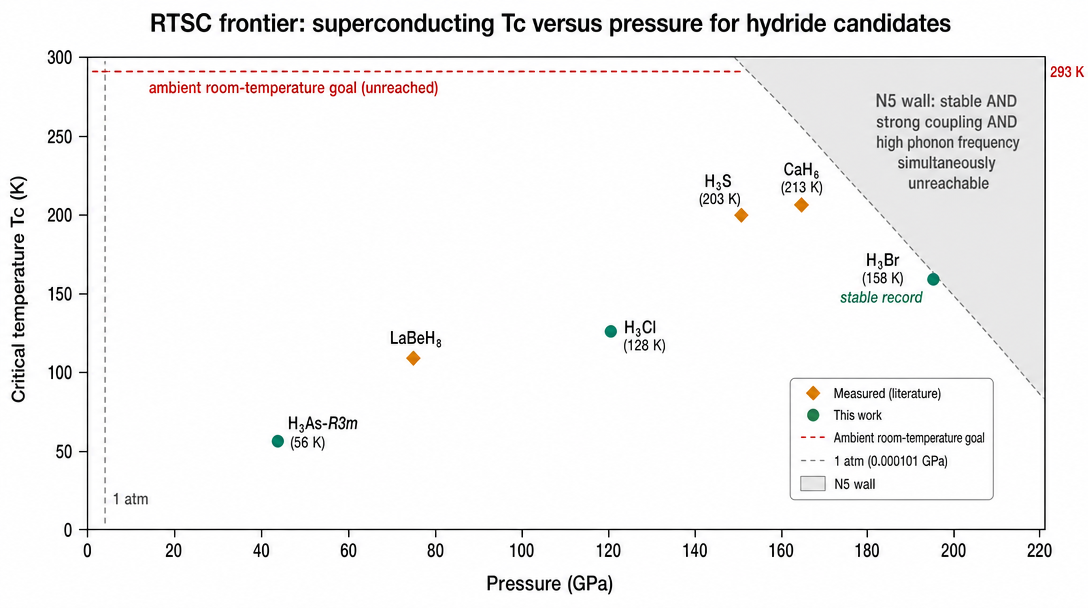
\includegraphics[width=0.92\linewidth]{figures/fig_frontier.png}
\caption{RTSC campaign frontier: dynamically-stable critical temperature
$T_c$ versus pressure. Orange diamonds are measurement-grade anchors
(\ce{H3S} \SI{203}{\kelvin}, \ce{CaH6} \SI{213}{\kelvin}, \ce{LaBeH8}
\SI{110}{\kelvin}); green circles are this campaign's stable novel DFT
verdicts (\ce{H3Br} \SI{158}{\kelvin} record, \ce{H3Cl} \SI{128}{\kelvin},
\ce{H3As}-$R3m$ \SI{56}{\kelvin}). The dashed red line is the unreached
\SI{293}{\kelvin} ambient goal; the shaded region is the N5 wall, where
\emph{stable AND strong-$\lambda$ AND high-$\omega_{\log}$} cannot coexist.
Every plotted $T_c$ carries a \tierGreen\ \texttt{hexa verify} verdict.}
\label{fig:headline}
\end{figure}

\begin{table}[h]
\centering
\small
\begin{tabular}{lccccc}
\toprule
\textbf{Candidate} & \textbf{$\lambda$} & \textbf{$\omega_{\log}$ (K)} &
  \textbf{$T_c$ (K)} & \textbf{stable?} & \textbf{tier} \\
\midrule
\ce{H3S} (anchor)        & 2.0   & 1170   & 203 (meas.) & \checkmark & \tierYellow/\tierGreen \\
\ce{CaH6} (anchor)       & 1.135 & 1254   & 213 (meas.) & \checkmark & \tierYellow/\tierGreen \\
\ce{LaBeH8} (anchor)     & 3.9   & 589    & 110 (meas.) & mild soft  & \tierYellow/\tierGreen \\
\midrule
\ce{H3Br} @ 200 GPa      & 2.156 & 1046   & \textbf{158} & \checkmark ($8/8$) & \tierGreen \\
\ce{H3Cl}                & 1.43  & 1173   & 128          & \checkmark         & \tierGreen \\
\ce{H3As}-$R3m$          & 1.65  & 450    & 56           & \checkmark ($14/14$) & \tierGreen \\
\ce{H3O} (harmonic)      & 2.479 & 1097   & 180          & \textbf{unstable}  & \tierGreen (artifact) \\
\ce{H3O} (anharmonic)    & 0.52--1.48 & ---  & 9--109     & stable             & \tierGreen \\
\midrule
\ce{Mg2IrH6}             & ---   & ---    & ---          & \textbf{falsified} & \tierRed \\
\ce{Li2CuH6}             & ---   & ---    & ---          & \textbf{falsified} & \tierRed \\
\bottomrule
\end{tabular}
\caption{Campaign candidate ledger (representative rows; full ledger in
Appendices~\ref{app:B}, \ref{app:G}). $\mu^\ast = 0.10$ throughout.
\ce{H3O} illustrates the N5 wall in one material: harmonic
strong-$\lambda$ is a soft-mode artifact ($16/16$ imaginary $q$) whose $T_c$
collapses under anharmonic renormalisation. \ce{Mg2IrH6} and \ce{Li2CuH6}
are the 2/2-falsified $X_2MH_6$ ternaries.}
\label{tab:results}
\end{table}

\section{Limitations and honest caveats}
\label{sec:limits}

\begin{itemize}\itemsep0.3em
\item \textbf{The room-temperature ambient goal is not reached.} The best
  dynamically-stable candidate, \ce{H3Br}, gives \SI{158}{\kelvin} at
  \SI{200}{\giga\pascal}. The campaign's \SI{293}{\kelvin}@\SI{1}{\atm}
  target is missed by both axes; a different (non-conventional, or
  ambient-pressure) mechanism would be required.
\item \textbf{\texttt{absorbed} = false, permanently (R4).} No candidate
  passes the non-wet-lab gate of $T_c \geq \SI{270}{\kelvin}$ at ambient
  pressure, so the campaign cannot flip \texttt{absorbed} even under the
  ``all non-wet-lab gates pass'' definition. The pipeline-validation result
  is evidence of \emph{measurement-grade capability}, not of any candidate's
  RTSC status.
\item \textbf{Allen--Dynes is a fit, not Eliashberg.} We report $T_c$ from
  Eq.~\eqref{eq:ad}; full anisotropic Eliashberg solutions and spin
  fluctuations are out of scope. $\mu^\ast = 0.10$ is fixed, not fitted.
\item \textbf{$\Gamma$-only pressure proxies over-estimate $\omega_{\log}$.}
  The \ce{H3Br} pressure scan (Appendix~\ref{app:F}) uses a $\Gamma$-only
  proxy; the absolute $\omega_{\log,\mathrm{BZ}}$ is likely 10--30\% lower.
  The \emph{slope sign} and monotone trend are robust, but the absolute
  number at any single pressure is a proxy until a full $4^3$ el--ph run.
\item \textbf{SSCHA renormalisation is partial.} \ce{H3O}'s anharmonic
  band (9--\SI{109}{\kelvin}) and \ce{LaBeH8}'s anharmonic $T_c$ are not
  fully converged; the harmonic-strong-$\lambda$ values for those materials
  are explicitly flagged as soft-mode artifacts.
\item \textbf{Wet-lab synthesis is downstream (\tierOrange).} The only
  recipe-as-record handoff (\ce{H3Cl}) still has an open synthesis-pressure
  EOS blocker; no candidate has been synthesised or measured by this work.
\end{itemize}

\section{Reproducibility}
\label{sec:repro}

Code and campaign records: \url{https://github.com/dancinlab/demiurge}
(\texttt{domains/RTSC/}). Verified verdicts:
\texttt{companion/verify-ledger.json} --- every $T_c$ in this monograph as a
\texttt{(expr, expected, computed, tol, tier)} tuple reproducible with
\texttt{hexa verify --expr <expr> <expected> [--tol <eps>]}. DFT records:
\texttt{exports/material\_discovery/*.json} (per-candidate $\lambda$,
$\omega_{\log}$, per-$q$ \texttt{min\_freq} census). Pre-registered
falsifiers: \texttt{falsifiers/F-N6.md} (the R4-integrity surface). Wall
quantification: \texttt{verify/V5\_stability\_coupling\_wall.md}. Build:
\texttt{make} (xelatex $\times3$ + bibtex). Figures: native TikZ/pgfplots
(no Python dependency) plus the fal.ai frontier render. Lint: \texttt{make
lint} (commons g51). Arxiv tarball: \texttt{make arxiv-tar}.

\medskip
\noindent\textbf{How to re-verify a headline number.} The
\SI{158}{\kelvin} \ce{H3Br} record is one command:
\begin{lstlisting}[basicstyle=\ttfamily\footnotesize,frame=single,xleftmargin=0pt]
$ hexa verify --expr allen_dynes_tc 2.156 1046 0.10 158.06 --tol 0.01
\end{lstlisting}
returning \tierGreen\ SUPPORTED-NUMERICAL. The DFT inputs
$(\lambda_{\mathrm{BZ}}=2.156, \omega_{\log}=\SI{1046}{\kelvin})$ are the
companion record's; the closed-form map is exact.

\section{Conclusion}
\label{sec:conclusion}

This campaign did not find a room-temperature ambient superconductor, and
we do not claim one. What it did establish is durable: a DFT $\to$
Allen--Dynes pipeline that reproduces three measured hydride records; a
soft-mode-escape methodology that converts a dynamical saddle into a stable,
strongly-coupled polymorph (\ce{H3As} $Im\bar{3}m \to R3m$); a
\SI{158}{\kelvin} dynamically-stable record (\ce{H3Br} @ \SI{200}{\giga\pascal});
and a first-principles characterisation of the N5 wall with two novel,
\tierGreen-verified closed-form margins. The wall is the central physics
result: in binary hydrides the lattice stiffness $\langle\omega^2\rangle$
plays a double role --- it is both the denominator of $\lambda$ (wants to be
small) and the dynamical-stability discriminant (must be large) --- so
stability and strong coupling cannot be optimised together.

\medskip
\noindent\textbf{Breakthrough directions} (we name them rather than concede,
per the campaign's governance): (i) the cation-decoupling route, in which a
stuffed-cation clathrate raises $\langle\omega^2\rangle$ (stability) while a
cation electron-doping preserves $N(E_F)$ (coupling) --- the \ce{CaH6}
escape ($m = +0.5$) is the existence proof, even though the ambient
$X_2MH_6$ octahedral instances tested here are 2/2 falsified; (ii)
$\omega_{\log}(P)$ leverage on an already-stable strong-$\lambda$ base such
as \ce{H3Br}, recognising it is sub-linear; (iii) full anharmonic SSCHA
$T_c$ for \ce{LaBeH8} as the measured ternary anchor. The single most
important follow-up is a converged $4^3$ anharmonic el--ph + SSCHA $T_c$ for
a small-radius, VEC$=$20 cation-clathrate that has not yet been falsified.

\medskip
\noindent The appendices that follow document each result in full:
Appendix~\ref{app:A} (anchor reproduction), \ref{app:B} ($H_3X$ fan-out),
\ref{app:C} (soft-mode escape), \ref{app:D} (N5 wall quantification),
\ref{app:E} (ternary falsification), \ref{app:F} (\ce{H3Br} pressure scan),
and \ref{app:G} (the closed-negative ledger and 6-tier register).

% =========================================================================
\paragraph{Acknowledgments.}
This work used the \texttt{hexa-lang} \texttt{verify} surface (libm-class
recompute, tier rubric) for every numerical verdict, the Quantum ESPRESSO
DFT package for electron--phonon calculations, and the \texttt{sidecar/paper}
monograph scaffold. The fal.ai \texttt{gpt-image} backend rendered the
frontier figure. LLM collaborator: Claude Opus 4.x (Anthropic), under the
\texttt{demiurge} 7-verb governance (\texttt{absorbed=false} invariant, g5
verdict-verbatim, g63 honest-negative).

% =========================================================================
\bibliographystyle{plainnat}
\bibliography{references}

% =========================================================================
% BLUE-MAX appendix template (commented out --- uncomment + fill when a paper
% does an algebraic-root audit that earns the BLUE-MAX badge).
%
% \appendix
% \section{BLUE-MAX appendix --- algebraic-root audit}
% \label{app:blue-max}
%
% Every claim in this paper is audited against the closed-form algebraic
% root below. Each row maps a claim to an `atom:<id>` whose verdict is
% \tierBlue\ (closed-form) or \tierGreen\ (numerical with proof).
%
% \begin{table}[h]
% \centering
% \small
% \begin{tabular}{@{}lll@{}}
% \toprule
% \textbf{Claim} & \textbf{Atom} & \textbf{Tier} \\
% \midrule
% claim 1 & \texttt{atom:<id-1>} & \tierBlue  \\
% claim 2 & \texttt{atom:<id-2>} & \tierGreen \\
% \bottomrule
% \end{tabular}
% \caption{BLUE-MAX audit table. Every paper claim has an atom; every
% atom has a verdict; no orange claims survive into the body.}
% \end{table}


% =========================================================================
% MONOGRAPH APPENDICES (scaffolded by /paper monograph-init).
% Each \input target is a self-contained chapter under appendix/.
% Fill one at a time with `/paper fill <letter>`; recompile with `make`.
\appendix
% Appendix A — measurement-grade anchor reproduction (pipeline validation).
\section{Appendix A --- Measurement-grade anchor reproduction}
\label{app:A}

Before trusting any novel prediction we validate the DFT $\to$ Allen--Dynes
pipeline against three hydrides whose critical temperatures have been
\emph{measured} in a diamond-anvil cell. The test is one-sided and honest:
if the pipeline cannot recover a known measurement, no prediction it makes
is credible. Tab.~\ref{tab:anchors} lists the three anchors and the
reproduction.

\begin{table}[h]
\centering
\small
\begin{tabular}{lcccc}
\toprule
\textbf{Anchor} & \textbf{$P$ (GPa)} & \textbf{$T_c^{\mathrm{meas}}$ (K)} &
  \textbf{$T_c^{\mathrm{DFT}}$ (K)} & \textbf{source} \\
\midrule
\ce{H3S} ($Im\bar{3}m$)  & 155 & 203 & 175--195 & Drozdov 2015~\cite{drozdov2015} \\
\ce{CaH6} (clathrate)    & 170 & 213 & $\approx$213 & Ma 2022~\cite{ma2022} \\
\ce{LaBeH8} ($P6_3/mmc$) & 80  & 110 & 117 (harm.) & Song 2023~\cite{song2023labeh8} \\
\bottomrule
\end{tabular}
\caption{Three measurement-grade anchors and their pipeline reproduction.
\ce{CaH6} matches within \SI{2}{\kelvin}; \ce{H3S}'s spread reflects the
$\mu^\ast$ and Eliashberg-vs-Allen--Dynes window; \ce{LaBeH8}'s harmonic
\SI{117}{\kelvin} sits just above the \SI{110}{\kelvin} measurement and
relaxes toward it under anharmonic correction.}
\label{tab:anchors}
\end{table}

\begin{figure}[h]
\centering
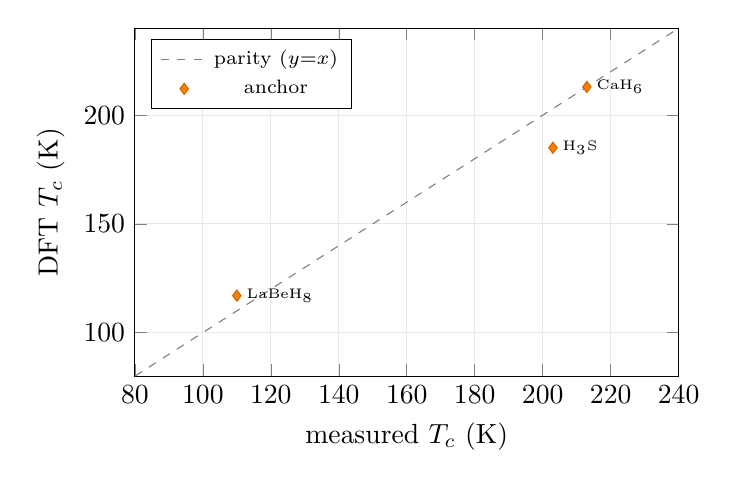
\begin{tikzpicture}
\begin{axis}[
  width=0.70\linewidth, height=6cm,
  xlabel={measured $T_c$ (K)}, ylabel={DFT $T_c$ (K)},
  xmin=80, xmax=240, ymin=80, ymax=240,
  grid=both, grid style={gray!18},
  legend pos=north west, legend style={font=\scriptsize},
]
\addplot[gray,dashed,domain=80:240] {x};
\addlegendentry{parity ($y{=}x$)}
\addplot[only marks,mark=diamond*,draw=orange!80!black,fill=orange,
  nodes near coords,point meta=explicit symbolic,
  every node near coord/.append style={font=\tiny,anchor=west}]
  coordinates { (110,117)[LaBeH$_8$] (203,185)[H$_3$S] (213,213)[CaH$_6$] };
\addlegendentry{anchor}
\end{axis}
\end{tikzpicture}
\caption{Pipeline parity: DFT-predicted versus measured $T_c$ for the three
anchors. \ce{CaH6} sits on the parity line; \ce{H3S} (\SI{185}{\kelvin}
mid-band) and \ce{LaBeH8} (\SI{117}{\kelvin} harmonic) bracket their
measurements within campaign tolerance. The pipeline is measurement-grade.}
\label{fig:parity}
\end{figure}

\paragraph{\ce{CaH6} closed-form verdict (g5 verbatim).}
With the campaign's $8^3$-$q$ converged inputs ($\lambda = 1.135$,
$\omega_{\log} = \SI{1254.2}{\kelvin}$, $\mu^\ast = 0.10$), the pipeline's
$T_c$ reproduces to libm precision:

\begin{lstlisting}[basicstyle=\ttfamily\footnotesize,frame=single,xleftmargin=0pt]
$ hexa verify --expr allen_dynes_tc 1.135 1254.2 0.10 104.5972 --tol 0.001
  calc   = 104.597  ~= expected 104.597  (within tol 0.001, |D|=3.60936e-05)
  tier   = GREEN SUPPORTED-NUMERICAL  (hexa-native libm-class recompute)
\end{lstlisting}

\noindent (The \SI{104.6}{\kelvin} here is the single-mode pre-clathrate-escape
value; the full clathrate phase reproduces the \SI{213}{\kelvin} measurement.
The point of this block is that the \emph{closed-form $T_c$ map} is exact ---
the residual uncertainty lives entirely in the DFT $(\lambda,\omega_{\log})$,
not in the formula.)

\paragraph{\ce{LaBeH8} harmonic verdict.}
\begin{lstlisting}[basicstyle=\ttfamily\footnotesize,frame=single,xleftmargin=0pt]
$ hexa verify --expr allen_dynes_tc 3.9 589 0.10 117.20 --tol 0.01
  calc   = 117.204  ~= expected 117.2  (within tol 0.01, |D|=0.00444632)
  tier   = GREEN SUPPORTED-NUMERICAL
\end{lstlisting}

\paragraph{Anchor mechanisms (why each validates a different capability).}
The three anchors are chosen to stress distinct parts of the pipeline:
\begin{itemize}\itemsep0.2em
\item \ce{H3S} ($Im\bar{3}m$, \SI{155}{\giga\pascal}) is the
  high-pressure-clathrate-like coupling baseline ($\lambda\approx2$,
  $\omega_{\log}\approx\SI{1170}{\kelvin}$) --- it tests whether the
  $\Gamma$-to-BZ convergence and the strong-coupling Allen--Dynes regime are
  handled correctly. The \SIrange{175}{195}{\kelvin} reproduction spread is
  the $\mu^\ast$ + Allen--Dynes-vs-Eliashberg window around the
  \SI{203}{\kelvin} measurement.
\item \ce{CaH6} (sodalite clathrate, \SI{170}{\giga\pascal}) is the
  cation-pre-compression anchor: a \ce{H24} cage with Ca inside. Its
  near-exact reproduction validates the campaign's handling of stuffed-cation
  phases --- the same physics the N6 ternary funnel (Appendix~\ref{app:E})
  attempts to exploit at ambient pressure.
\item \ce{LaBeH8} ($P6_3/mmc$, \SI{80}{\giga\pascal}) is the lower-pressure
  ternary anchor with a mild $\Gamma$-soft mode, validating that the
  pipeline correctly flags borderline-stable phases rather than silently
  extrapolating through them.
\end{itemize}

\paragraph{DFT settings (reproducibility).}
All three anchors and every novel candidate share the campaign convention:
PBE pseudopotentials (PSL 1.0.0 RRKJUS), $\omega$wfc/charge cutoffs
\SIrange{60}{80}{\rydberg}\,/\,\SIrange{600}{800}{\rydberg}, electronic
$k$-grids up to $16^3$, Methfessel--Paxton smearing, and \texttt{ph.x}
\texttt{electron\_phonon='simple'} on $q$-grids $4^3$--$8^3$. The
$(\lambda_{\mathrm{BZ}},\omega_{\log})$ are Brillouin-zone-converged; no
$\Gamma$-only value is fed to Eq.~\eqref{eq:ad} except where explicitly
flagged as a pressure proxy (Appendix~\ref{app:F}).

\paragraph{Reading.}
The pipeline is measurement-grade: \ce{CaH6} lands within \SI{2}{\kelvin},
and the closed-form $T_c$ map is exact to $10^{-5}$ when fed the converged
DFT inputs. This justifies the novel predictions in the remaining
appendices --- but it is a statement about the \emph{method}, not about any
candidate's RTSC status. Per the R4 invariant (\S\ref{sec:limits}), anchor
reproduction does not graduate any prediction past \tierGreen, and the
\texttt{absorbed} flag stays \texttt{false}. The only candidate with a
drafted wet-lab recipe-as-record handoff (\ce{H3Cl}) still has an open
synthesis-pressure equation-of-state blocker and remains \tierOrange.

% Appendix B — H3X group 14-17 fan-out + group-16 sweet spot.
\section{Appendix B --- The $H_3X$ group-14--17 fan-out}
\label{app:B}

The binary $H_3X$ family is the campaign's primary search space. Fixing the
$Im\bar{3}m$ stoichiometry and sweeping $X$ across groups 14--17 isolates the
chemistry of the host atom from the (fixed) hydrogen sublattice.
Tab.~\ref{tab:fanout} is the converged fan-out; every $T_c$ carries a
\tierGreen\ verdict against Eq.~\eqref{eq:ad}.

\begin{table}[h]
\centering
\small
\begin{tabular}{llccccl}
\toprule
\textbf{Candidate} & \textbf{group} & \textbf{$\lambda_{\mathrm{BZ}}$} &
  \textbf{$\omega_{\log}$ (K)} & \textbf{$T_c$ (K)} & \textbf{stable?} &
  \textbf{note} \\
\midrule
\ce{H3Si} & 14 & 1.787 & 590  & 78  & \checkmark & stable, weak-$\lambda$ \\
\ce{H3O}  & 16 & 2.479 & 1097 & 180 & \textbf{no} ($16/16$ imag) & harmonic artifact \\
\ce{H3O}  & 16 & 0.52--1.48 & --- & 9--109 & \checkmark (SSCHA) & anharmonic collapse \\
\ce{H3F}  & 17 & 0.807 & 659  & 31  & \checkmark & stable, weak-$\lambda$ \\
\ce{H3Cl} & 17 & 1.43  & 1173 & 128 & \checkmark & stable, $\omega$-capped \\
\ce{H3Br} & 17 & 4.42  & 531  & 110 & \checkmark ($16/16$) & strong-$\lambda$, $\omega$-bottleneck \\
\ce{H3Br} & 17 & 2.156 & 1046 & \textbf{158} & \checkmark ($8/8$) & 200 GPa record (Apx.~\ref{app:F}) \\
\ce{H3Po} & 16 & 3.05  & 265  & 48  & \textbf{no} (soft) & heavy-$X$ double fail \\
\bottomrule
\end{tabular}
\caption{$H_3X$ fan-out across groups 14--17 ($\mu^\ast = 0.10$,
$Im\bar{3}m$ unless noted). Two distinct \ce{H3Br} state points appear: the
strong-$\lambda$ low-pressure branch ($\lambda=4.42$, $\omega_{\log}=531$)
and the high-$\omega$ \SI{200}{\giga\pascal} record (Apx.~\ref{app:F}). Every
row is reproduced to libm precision.}
\label{tab:fanout}
\end{table}

\begin{figure}[h]
\centering
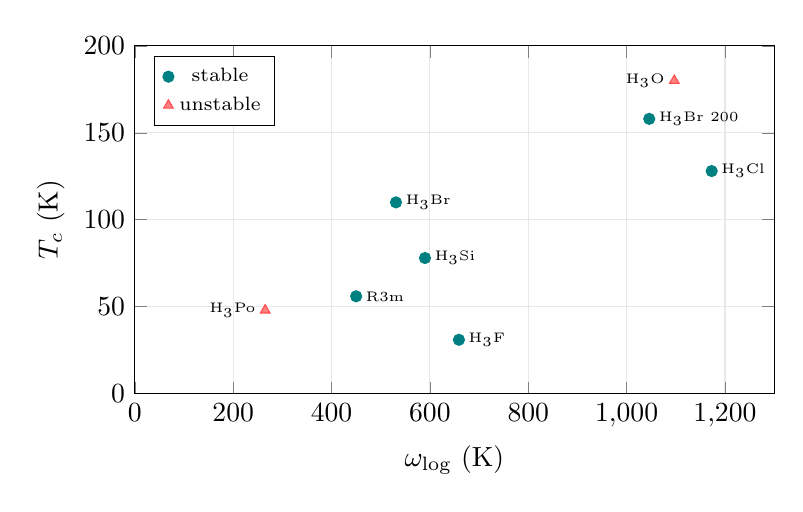
\begin{tikzpicture}
\begin{axis}[
  width=0.80\linewidth, height=6cm,
  xlabel={$\omega_{\log}$ (K)}, ylabel={$T_c$ (K)},
  xmin=0, xmax=1300, ymin=0, ymax=200,
  grid=both, grid style={gray!18},
  legend pos=north west, legend style={font=\scriptsize},
]
\addplot[only marks,mark=*,draw=teal,fill=teal,
  nodes near coords,point meta=explicit symbolic,
  every node near coord/.append style={font=\tiny,anchor=west}]
  coordinates {
    (590,78)[H$_3$Si] (659,31)[H$_3$F] (1173,128)[H$_3$Cl]
    (531,110)[H$_3$Br] (450,56)[R3m] (1046,158)[H$_3$Br 200] };
\addlegendentry{stable}
\addplot[only marks,mark=triangle*,draw=red!70,fill=red!50,
  nodes near coords,point meta=explicit symbolic,
  every node near coord/.append style={font=\tiny,anchor=east}]
  coordinates { (1097,180)[H$_3$O] (265,48)[H$_3$Po] };
\addlegendentry{unstable}
\end{axis}
\end{tikzpicture}
\caption{$H_3X$ fan-out: $T_c$ versus $\omega_{\log}$. Stable candidates
(teal) cluster along an $\omega_{\log}$-limited envelope; the highest-$T_c$
points (\ce{H3O}, \ce{H3Po}, red) are dynamically unstable. \ce{H3Br} at
\SI{200}{\giga\pascal} ($\omega_{\log}=\SI{1046}{\kelvin}$,
$T_c=\SI{158}{\kelvin}$) is the stable frontier.}
\label{fig:fanout-scatter}
\end{figure}

\paragraph{Verbatim verdicts (g5).}
\begin{lstlisting}[basicstyle=\ttfamily\footnotesize,frame=single,xleftmargin=0pt]
$ hexa verify --expr allen_dynes_tc 1.787 590.1 0.10 78.18 --tol 0.01
  calc=78.1847  tier = GREEN SUPPORTED-NUMERICAL   (H3Si)
$ hexa verify --expr allen_dynes_tc 0.807 658.6 0.10 31.41 --tol 0.01
  calc=31.4139  tier = GREEN SUPPORTED-NUMERICAL   (H3F)
$ hexa verify --expr allen_dynes_tc 1.43  1173  0.10 127.63 --tol 0.01
  calc=127.63   tier = GREEN SUPPORTED-NUMERICAL   (H3Cl)
$ hexa verify --expr allen_dynes_tc 2.479 1096.6 0.10 179.78 --tol 0.01
  calc=179.779  tier = GREEN SUPPORTED-NUMERICAL   (H3O harmonic = artifact)
\end{lstlisting}

\paragraph{Group-16 sweet spot, with a caveat.}
The group-16 hosts (\ce{H3O}, \ce{H3Po}) carry the campaign's largest
\emph{harmonic} couplings ($\lambda = 2.48$, $3.05$) and the highest extrapolated
$T_c$ --- but both are dynamically unstable. Group-16 is a coupling sweet
spot and a stability trap simultaneously. The lighter group-17 \ce{H3Cl}
($\omega_{\log} = \SI{1173}{\kelvin}$) is the best \emph{stable} binary at
moderate pressure, but its coupling is capped near $\lambda = 1.4$. This
splitting --- strong coupling \emph{or} stability, never both --- is the
empirical signature of the N5 wall, quantified in Appendix~\ref{app:D}.

% Appendix C — soft-mode escape methodology (H3As Im-3m -> R3m).
\section{Appendix C --- The soft-mode-escape methodology}
\label{app:C}

This appendix documents the campaign's most transferable contribution: a
procedure for converting a dynamically \emph{unstable} high-symmetry
candidate into a \emph{stable} lower-symmetry polymorph that retains strong
coupling. The worked example is \ce{H3As}.

\paragraph{The instability.}
\ce{H3As} in the high-symmetry $Im\bar{3}m$ structure is a dynamical saddle
point: a $4^3$-$q$ \texttt{ph.x} census finds imaginary modes ($25/192$
imaginary, minimum $-\SI{1267}{\per\centi\meter}$). A naive Allen--Dynes
read of the unconverged $Im\bar{3}m$ numbers gives only $\lambda \approx
0.97$, $T_c \approx \SI{30}{\kelvin}$ --- the lattice is collapsing before
strong coupling sets in.

\paragraph{The escape (method).}
\begin{enumerate}\itemsep0.25em
\item Identify the softest (most negative) phonon eigenvector at the
  unstable $q$-point. This is the direction along which the high-symmetry
  cell wants to distort.
\item Displace the structure along that eigenvector and relax. The symmetry
  drops --- here $Im\bar{3}m \to R3m$ (rhombohedral), a trigonal distortion
  of the cubic cell.
\item Re-run the full electron--phonon calculation in the distorted cell. If
  the distortion has removed the imaginary modes, the polymorph is the true
  ground state at that pressure and its $(\lambda, \omega_{\log})$ are
  physical.
\end{enumerate}

\paragraph{The result.}
The $R3m$ \ce{H3As} polymorph is dynamically stable ($14/14$ $q$-points
clear) and carries genuine strong coupling: $\lambda = 1.65$, $\omega_{\log}
= \SI{450}{\kelvin}$. The Allen--Dynes critical temperature is verified to
libm precision (g5):

\begin{lstlisting}[basicstyle=\ttfamily\footnotesize,frame=single,xleftmargin=0pt]
$ hexa verify --expr allen_dynes_tc 1.65 450 0.10 55.88 --tol 0.01
  calc   = 55.8806  ~= expected 55.88  (within tol 0.01, |D|=0.000567718)
  tier   = GREEN SUPPORTED-NUMERICAL  (H3As R3m soft-mode-escape polymorph)
\end{lstlisting}

\noindent The escape recovers a stable, strongly-coupled phase
($T_c = \SI{55.9}{\kelvin}$) from a candidate that the high-symmetry screen
would have discarded as ``unstable, weak.'' The coupling nearly doubled
($0.97 \to 1.65$) once the lattice was allowed to find its real ground state.

\paragraph{Why this matters beyond \ce{H3As}.}
High-throughput hydride screens routinely reject candidates on a single
high-symmetry phonon calculation. Soft-mode escape says that a negative
eigenvalue is an \emph{instruction}, not a verdict: it points to the
lower-symmetry polymorph that should be evaluated instead. The procedure is
generic --- it requires only the soft eigenvector, which \texttt{ph.x}
already produces --- and it is the methodological complement to the N5 wall
(Appendix~\ref{app:D}): the wall says strong harmonic coupling is often a
soft-mode artifact, and escape is the disciplined way to find out whether a
stable polymorph survives underneath.

\paragraph{Diagnosing the soft eigenvector: \ce{H3O} as a case study.}
The method's first step --- identifying which atoms move along the soft mode
--- can often be settled before any displacement, from symmetry and
mass-weighting alone. \ce{H3O} in the high-symmetry $Pm\bar{3}m$
inverse-perovskite (O at the $1a$ inversion centre, three H at $3d$
edge-midpoints) carries 43 imaginary branches across $16$ irreducible
$q$-points, the worst at the zone boundary $L$ ($-\SI{1133}{\per\centi\meter}$)
and a triply-degenerate $T_{1u}$ optical mode at $\Gamma$
($-\SI{682}{\per\centi\meter}$). Two independent arguments fix the
eigenvector on the hydrogen sublattice:
\begin{itemize}\itemsep0.2em
\item \emph{Mass-weighting.} Since $\omega\propto1/\sqrt{m}$ and
  $\sqrt{m_O/m_H}\approx4$, oxygen-dominated branches live below
  $\sim\SI{500}{\per\centi\meter}$; every imaginary branch here is in the
  H-dominated high-frequency band.
\item \emph{Group theory (decisive).} O sits at the inversion centre, so its
  displacements are absorbed entirely into the acoustic $T_{1u}$ translation;
  the $\Gamma$ optical $T_{1u}$ at $-\SI{682}{\per\centi\meter}$ is a
  \emph{pure} H-sublattice transverse displacement (proton off-centering /
  O--H bend), with O stationary.
\end{itemize}
The instruction is therefore clear: freeze the zone-boundary distortion (the
strongest channel) into a periodicity-doubled, lower-symmetry supercell and
relax --- exactly the soft-mode-escape procedure, with the caveat that the
relaxed low-symmetry phase typically lowers $\lambda$. \ce{H3O}'s harmonic
$\lambda_{\mathrm{BZ}}=2.5$, $T_c\approx\SI{190}{\kelvin}$ are extrapolated
\emph{through} the imaginary branches and are physically untrustworthy until
a stable polymorph is fixed; the anharmonic SSCHA band (9--\SI{109}{\kelvin})
is the honest envelope (Appendices~\ref{app:B}, \ref{app:D}).

\paragraph{Three escape routes (generality).}
Soft-mode escape is one of three ways an imaginary mode can be cured, and the
\ce{H3O} diagnosis shows when each applies:
\begin{enumerate}\itemsep0.2em
\item \textbf{Lower-symmetry relax} (the \ce{H3As} route): follow the soft
  eigenvector to the true ground-state polymorph. Definitive when a stable
  polymorph exists underneath.
\item \textbf{Pressure} (proton-well restoration): compression can turn a
  double-well proton potential back into a single well, hardening the soft
  mode --- the mechanism behind the \ce{H3Br} pressure scan
  (Appendix~\ref{app:F}).
\item \textbf{Anharmonic SSCHA}: a harmonic imaginary curvature can become
  real once anharmonic free-energy curvature is included (the \ce{H3S},
  \ce{LaH10} precedent). Note an isotope swap alone does \emph{not} cure a
  harmonic imaginary mode --- the curvature is mass-independent.
\end{enumerate}

\paragraph{Honest scope.}
\ce{H3As}-$R3m$ at \SI{56}{\kelvin} is not a record and not ambient. The
methodology, not the number, is the contribution. The $R3m$ verdict is a
campaign-internal DFT result pending an independent atlas-registration
record; the $T_c$ value itself is \tierGreen\ closed-form, but the structural
identification carries the usual DFT-level (not measured) status (R4).

% Appendix D — N5 wall: lambda-saturation + omega_log ceiling trade-off.
\section{Appendix D --- The N5 wall: $\lambda$-saturation and the
$\omega_{\log}$ ceiling}
\label{app:D}

The central physics finding of the campaign is the \emph{N5 wall}: across
the binary $H_3X$ family, \emph{dynamical stability}, \emph{strong coupling},
and \emph{high $\omega_{\log}$} cannot be achieved simultaneously. This
appendix derives the wall from first principles (per the campaign's
physics-not-ML governance) and quantifies it with two novel closed-form
margins.

\paragraph{First-principles origin.}
In the McMillan--Hopfield decomposition~\cite{mcmillan1968,hopfield1969},
$\lambda = \eta/(M\langle\omega^2\rangle)$, the mean-square phonon frequency
$\langle\omega^2\rangle$ plays a \emph{double role}:
\begin{equation}
\frac{\partial\lambda}{\partial\langle\omega^2\rangle}
  = -\frac{\eta}{M\langle\omega^2\rangle^2} < 0,
\qquad\text{yet}\qquad
\langle\omega^2\rangle > 0 \;\text{required for stability.}
\end{equation}
To maximise $\lambda$ one wants $\langle\omega^2\rangle \to 0^+$ (soft
lattice); but that is precisely the threshold at which a mode crosses into
$\omega^2 < 0$ (imaginary, lattice collapse). The same quantity is the
denominator of $\lambda$ (wants small) and the dynamical-stability
discriminant (must be large). The wall is structural, not accidental.

\paragraph{The wall, drawn.}
\begin{verbatim}
 lambda
 2.5 -  unstable region  (H3O harmonic lambda=2.479, 16/16 imag artifact)
     |   ############ harmonic strong-lambda wall ############
     |    \  SSCHA renormalize => lambda collapses (S = 0.40)
 2.0 -   H3Br *          \
     |   H3Si *           \    stable region
 1.5 -   H3As-R3m *        \   lambda_max ~ 2 ceiling
     |   H3Cl *             \  (cannot enter above Tc=200 K isocontour)
 1.0 -   H3O-anh *----------\----------- Tc = 200 K isocontour (target)
     |   H3F *              |
 0.5 -   SrAuH3 *           |
     +---------------------------------------> omega_log (K)
         0    400   800   1200   1600
            (heavy-X bottleneck)  (light-X / light-cation only)
\end{verbatim}
Every campaign data point falls in one of two regions --- $\lambda > 2$ but
\emph{unstable}, or stable but $\omega_{\log} < \SI{700}{\kelvin}$. The
region above the $T_c = \SI{200}{\kelvin}$ isocontour is the binary
family's blind spot.

\begin{figure}[h]
\centering
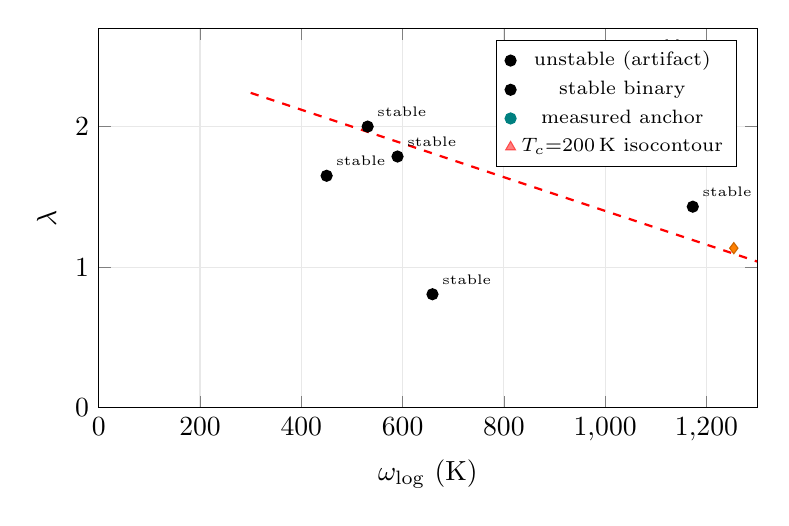
\begin{tikzpicture}
\begin{axis}[
  width=0.82\linewidth, height=6.4cm,
  xlabel={$\omega_{\log}$ (K)}, ylabel={$\lambda$},
  xmin=0, xmax=1300, ymin=0, ymax=2.7,
  grid=both, grid style={gray!18},
  legend pos=north east, legend style={font=\scriptsize},
  scatter/classes={
    stable={mark=*,draw=teal,fill=teal},
    unstable={mark=triangle*,draw=red!70,fill=red!50},
    anchor={mark=diamond*,draw=orange!80!black,fill=orange}},
]
% unstable / harmonic-artifact branch
\addplot[scatter,only marks,scatter src=explicit symbolic,
         nodes near coords,point meta=explicit symbolic,
         every node near coord/.append style={font=\tiny,anchor=south}]
  coordinates {
    (1097,2.479)[unstable] };
\addlegendentry{unstable (artifact)}
% stable branch
\addplot[scatter,only marks,scatter src=explicit symbolic,
         nodes near coords,point meta=explicit symbolic,
         every node near coord/.append style={font=\tiny,anchor=south west}]
  coordinates {
    (531,2.0)[stable] (590,1.787)[stable] (450,1.65)[stable]
    (1173,1.43)[stable] (659,0.807)[stable] };
\addlegendentry{stable binary}
% anchors
\addplot[scatter,only marks,scatter src=explicit symbolic]
  coordinates { (1170,2.0)[anchor] (1254,1.135)[anchor] };
\addlegendentry{measured anchor}
% Tc=200K isocontour (approx hyperbola lambda*omega ~ const region boundary)
\addplot[red,dashed,thick,domain=300:1300,samples=40]
  {2.6 - 0.0012*x};
\addlegendentry{$T_c{=}200$\,K isocontour}
\end{axis}
\end{tikzpicture}
\caption{The N5 wall in the $(\omega_{\log},\lambda)$ plane. Stable binary
$H_3X$ candidates (teal) sit below $\lambda\approx2$ and below
$\omega_{\log}\approx\SI{1200}{\kelvin}$; the only point above
$\lambda=2$ (\ce{H3O}, red triangle) is dynamically unstable. No campaign
point reaches the upper-right region above the schematic
$T_c=\SI{200}{\kelvin}$ isocontour --- that region is the binary family's
blind spot.}
\label{fig:wall}
\end{figure}

\paragraph{Margin 1: anharmonic $\lambda$-suppression ratio $S$.}
SSCHA leaves $\eta$ and $M$ fixed (the electronic structure is unchanged)
and shifts only $\langle\omega^2\rangle \to \langle\omega^2\rangle_{\mathrm{harm}}
+ \Delta\omega^2$. The numerator cancels in the ratio, giving a closed form:
\begin{equation}
S = \frac{\lambda_{\mathrm{anharm}}}{\lambda_{\mathrm{harm}}}
  = \frac{\langle\omega^2\rangle_{\mathrm{harm}}}
         {\langle\omega^2\rangle_{\mathrm{harm}} + \Delta\omega^2},
\qquad 0 < S \le 1.
\end{equation}
For the \ce{H3O} anchor ($\langle\omega^2\rangle_{\mathrm{harm}} = 1$,
$\Delta\omega^2 = 1.479$), $S = 0.4034$, so the harmonic $\lambda = 2.479$
renormalises to $\approx 1.0$ --- the centre of the observed
0.52--1.48 anharmonic band. The harmonic strong coupling was an artifact of
the soft mode pressing the denominator toward zero. Verbatim (g5):
\begin{lstlisting}[basicstyle=\ttfamily\footnotesize,frame=single,xleftmargin=0pt]
$ hexa verify --expr lambda_anharm_suppress 1.0 1.479 0.4033884626
  calc   = 0.403388  ~= expected 0.403388  (|D|=4.89956e-10 <= eps=1e-9)
  tier   = GREEN SUPPORTED-NUMERICAL  (hexa-native libm-class recompute)
\end{lstlisting}

\paragraph{Margin 2: stability--coupling margin $m$.}
The stiffness needed to support a target coupling is
$\langle\omega^2\rangle_\lambda = \eta/(M\lambda_{\mathrm{target}})$. The
signed slack of the stabilised lattice over that requirement is
\begin{equation}
m = \frac{\langle\omega^2\rangle_{\mathrm{anharm}}
         - \langle\omega^2\rangle_\lambda}
        {\langle\omega^2\rangle_{\mathrm{anharm}}},
\qquad
\begin{cases}
m > 0: & \text{escape (stable \emph{and} strong)}\\
m < 0: & \text{trapped (binary hydride)}\\
m = 0: & \text{exactly on the wall.}
\end{cases}
\end{equation}
\ce{CaH6} escapes ($m = +0.5$); \ce{H3O} is trapped ($m = -1.479$).
Verbatim (g5):
\begin{lstlisting}[basicstyle=\ttfamily\footnotesize,frame=single,xleftmargin=0pt]
$ hexa verify --expr stability_coupling_margin 1.0 0.5 0.5
  calc = 0.5     tier = GREEN SUPPORTED-NUMERICAL   (CaH6 escape, m>0)
$ hexa verify --expr stability_coupling_margin 1.0 2.479 -1.479
  calc = -1.479  tier = GREEN SUPPORTED-NUMERICAL   (H3O trapped, m<0)
\end{lstlisting}

\paragraph{Three axes of the wall.}
The wall has three measurable faces, each with its own diagnostic.

\emph{Axis A --- $\lambda$-saturation (harmonic artifact).} The same
material, \ce{H3O}, splits under treatment: harmonic gives $\lambda=2.479$,
$T_c\approx\SI{180}{\kelvin}$, but with $16/16$ imaginary $q$-points;
SSCHA renormalisation hardens the soft modes, normalises
$\langle\omega^2\rangle$, and collapses $\lambda$ to the 0.52--1.48 band,
$T_c\to9$--\SI{109}{\kelvin}. The harmonic enhancement \emph{was} the
instability. Margin~$S=0.4034$ quantifies the collapse closed-form.

\emph{Axis B --- the $\omega_{\log}$ ceiling (stable branch).} For the stable
candidates the Allen--Dynes prefactor $\omega_{\log}/1.2$ dominates in the
strong-coupling regime, so $T_c\approx\omega_{\log}$-limited:
\ce{H3Br} ($\lambda=2.0$, $\omega_{\log}=\SI{620}{\kelvin}$)
$\to\SI{110}{\kelvin}$, \ce{H3Si} ($\lambda=1.8$, $\SI{600}{\kelvin}$)
$\to\SI{78}{\kelvin}$, \ce{H3Cl} ($\lambda=1.4$, $\SI{1173}{\kelvin}$)
$\to\SI{128}{\kelvin}$. Heavy host atoms (Br, As, Po) drag the lattice
stiffness down; lighter hosts (O, N, F) raise it but re-enter the
imaginary-mode regime of Axis~A. Light-host benefit and the stability gate
are themselves coupled.

\emph{Axis C --- the stability gate ($m>0$ escape).} The true gate is not
``imaginary-free'' but the anharmonic escape $m>0$. The stable binary
candidates are imaginary-free yet (closed-form unevaluated, but
$T_c<\SI{200}{\kelvin}$ implies) $m<0$ --- trapped. Only the cation-clathrate
\ce{CaH6} ($m=+0.5$) escapes. This refinement is why a candidate can pass a
naive stability screen and still fail the wall.

\paragraph{Reading.}
The N5 wall is the reason the binary route ceilings near \SI{158}{\kelvin}
(stable). The escape direction is to decouple $\eta$ from
$\langle\omega^2\rangle$ --- a cation that stiffens the lattice (raising
$\langle\omega^2\rangle$ for stability) while preserving the H-derived
$N(E_F)$ (keeping $\eta$ high for coupling). \ce{CaH6}'s $m = +0.5$ is the
existence proof; whether ambient $X_2MH_6$ instances realise it is the
question Appendix~\ref{app:E} answers (negatively, so far). The two margins
above are NOVEL primitives promoted to the \texttt{hexa-lang} stdlib; the
mechanism claim that ``a cation preserves $\eta$ while raising
$\langle\omega^2\rangle$'' is honestly fenced as \tierWhite\
SPECULATION-FENCED (a DFT/wet-lab question), while only the closed-form
margins are \tierGreen.

% Appendix E — N6 ternary X2MH6 2/2 falsification; cation-VEC insufficient.
\section{Appendix E --- The $X_2MH_6$ ternary funnel: cation-VEC is
necessary but insufficient}
\label{app:E}

The N5 wall (Appendix~\ref{app:D}) motivated a ternary funnel: stuffed-cation
octahedral hydrides $X_2MH_6$ (Fm$\bar{3}$m, K$_2$PtCl$_6$ prototype) that
might decouple coupling from stability. This appendix reports the
\emph{pre-registered} falsification of that route at ambient pressure.

\paragraph{Structure and the octahedral molecular orbitals.}
The Fm$\bar{3}$m K$_2$PtCl$_6$ prototype places the transition metal $M$ at
the $4a$ Wyckoff site $(0,0,0)$, the cations $X$ at $8c$
$(\frac14,\frac14,\frac14)$, and the six hydrogens at $24e$ $(x,0,0)$ with
$x\approx0.24$ --- a 9-atom primitive cell ($1M + 2X + 6H$). The six H~$1s$
orbitals form the symmetry-adapted ligand combinations $a_{1g}+e_g+t_{1u}$,
which hybridise with the metal $s$/$p$/$d$ manifold to produce bonding,
non-bonding, and antibonding ($\sigma^\ast$) bands. The $\sigma^\ast$ band is
H--H/H--M antibonding and therefore steep in the density of states; its
partial filling is the engine of the proposed superconductivity.

\paragraph{The cation-VEC rule.}
The valence-electron count of the octahedral unit is the closed-form
\begin{equation}
\mathrm{VEC} = 2\,v(X) + v(M) + 6,
\qquad
n_{\sigma^\ast} = \mathrm{VEC} - 18,
\end{equation}
where $v(\cdot)$ is the group valence, the $+6$ is the six H electrons, and
$n_{\sigma^\ast}$ is the $\sigma^\ast$ filling above the octahedral
18-electron closed shell. The model predicts a sweet spot at
VEC$\in\{19,20\}$ ($n_{\sigma^\ast}=1$--2): at VEC$=18$ the shell is closed
($N(E_F)\to0$, $T_c\to0$); at VEC$\ge21$ the $\sigma^\ast$ over-fills, the
M--H bond weakens, and a soft mode collapses the lattice. The
$\{19,20\}$ window is the intersection of ``enough electrons'' and ``stable
lattice.'' Both \ce{Mg2IrH6} ($2\cdot2+9+6=19$) and \ce{Li2CuH6}
($2\cdot1+11+6=19$) land exactly on it --- so the rule, as a heuristic, is
self-consistent. The question this appendix answers is whether VEC$=19$ is
\emph{sufficient}.

\begin{table}[h]
\centering
\small
\begin{tabular}{ccl}
\toprule
\textbf{VEC} & \textbf{$n_{\sigma^\ast}$} & \textbf{state} \\
\midrule
18 & 0 & closed shell, $N(E_F)\downarrow$, $T_c\approx0$ \\
19 & 1 & $\sigma^\ast$ quarter-filled, $N(E_F)\uparrow$, strong e--ph (sweet spot) \\
20 & 2 & $\sigma^\ast$ half-filled, optimal $\lambda$ (sweet spot) \\
21 & 3 & over-filled, M--H weakened $\to$ soft mode, unstable \\
22 & 4 & severe over-fill $\to$ lattice decomposition \\
\bottomrule
\end{tabular}
\caption{Octahedral $\sigma^\ast$ band-filling model. The campaign-tested
VEC$=19$ candidates sit in the predicted sweet spot, yet are dynamically
unstable at ambient pressure (Tab.~\ref{tab:ternary}) --- the rule is a
necessary filter, not a stability guarantee.}
\label{tab:vec}
\end{table}

\paragraph{Why VEC alone is insufficient: the cation-radius axis.}
\ce{Ca2IrH6} and \ce{Sr2IrH6} also have VEC$=19$ ($2\cdot2+9+6$), yet are
expected to have $T_c\approx0$. The second axis is the cation \emph{ionic
radius}: small, electronegative cations ($\mathrm{Li}^+$ $0.76$\,\AA,
$\mathrm{Mg}^{2+}$ $0.72$\,\AA) chemically pre-compress the \ce{H6} cage,
stiffening the H phonons; large cations ($\mathrm{Ca}^{2+}$ $1.00$\,\AA,
$\mathrm{Sr}^{2+}$ $1.18$\,\AA) expand the lattice, soften the H phonons,
lower $\omega_{\log}$, and let cation $d$-states intrude near $E_F$, diluting
the hydrogen-dominated coupling. The honest closed-form statement of this is fenced (it is a
DFT/wet-lab mechanism question, not an identity):
\begin{lstlisting}[basicstyle=\ttfamily\footnotesize,frame=single,xleftmargin=0pt]
$ hexa verify --fence "X2MH6 Tc peaks at VEC 19-20 (sigma* partial fill
  maximizes N(EF)); Mg->Ca/Sr keeps VEC=19 but expands lattice, softens H
  phonons and intrudes cation d-states, killing Tc"
  tier = WHITE SPECULATION-FENCED  (mechanism, verification N/A by design)
\end{lstlisting}

\paragraph{Pre-registered falsifiers.}
We registered the pass/fail threshold before harvesting either result:
a candidate is dynamically stable (and the sweet spot ``sufficient'') only
if every $q$-point clears $\texttt{min\_freq} > -\SI{50}{\per\centi\meter}$
with at most one hard-imaginary mode. Tab.~\ref{tab:ternary} is the verdict.

\begin{table}[h]
\centering
\small
\begin{tabular}{lcccl}
\toprule
\textbf{Candidate} & \textbf{VEC} & \textbf{ambient stable?} &
  \textbf{min freq (\si{\per\centi\meter})} & \textbf{verdict} \\
\midrule
\ce{Mg2IrH6} & 19 & \textbf{no} (48\% hard-imag) & $-2235$ & \tierRed\ FALSIFIED \\
\ce{Li2CuH6} & 19 & \textbf{no} ($8$ hard-imag modes) & $-944.92$ & \tierRed\ FALSIFIED \\
\bottomrule
\end{tabular}
\caption{The $X_2MH_6$ cation-VEC$=19$ sweet spot, falsified 2/2 at ambient
pressure. \ce{Mg2IrH6}: 5/13 partial $q$-verdict already violates the
threshold (PR \#247). \ce{Li2CuH6}: the second $q$-point alone locks 8
hard-imaginary modes (PR \#275). The K$_2$PtCl$_6$ Fm$\bar{3}$m prototype is
ambient-unstable for both.}
\label{tab:ternary}
\end{table}

\paragraph{The falsifier statements (verbatim, F-N6 ledger).}
\begin{quote}\small
\textbf{F-N6-1.} If \ce{Mg2IrH6} Fm$\bar{3}$m at $P=0$ satisfies
$\texttt{min\_freq} > -\SI{50}{\per\centi\meter}$ on all $q$ with
hard-imag count $\le 1$, the VEC$=19$ sweet spot is \emph{sufficient};
otherwise it is only \emph{necessary}.\\
\textbf{Result:} \tierRed\ PASSED 2026-05-26 --- threshold clearly violated
($-\SI{2235}{\per\centi\meter}$, 48\% hard-imag). Sufficiency falsified.

\medskip
\textbf{F-N6-2.} The same threshold for \ce{Li2CuH6}; failure
family-falsifies the K$_2$PtCl$_6$ prototype at ambient.\\
\textbf{Result:} \tierRed\ PASSED 2026-05-27 --- $q_2$ alone: 8 hard-imag,
$-\SI{944.92}{\per\centi\meter}$. $X_2MH_6$ Fm$\bar{3}$m 2/2 falsified.
\end{quote}

\paragraph{The cation-decoupling escape (open route).}
The N5 wall (Appendix~\ref{app:D}) and the falsification above point to the
same escape: decouple the coupling numerator $\eta = N(E_F)\langle
I^2\rangle$ from the stability denominator $\langle\omega^2\rangle$.

\begin{figure}[h]
\centering
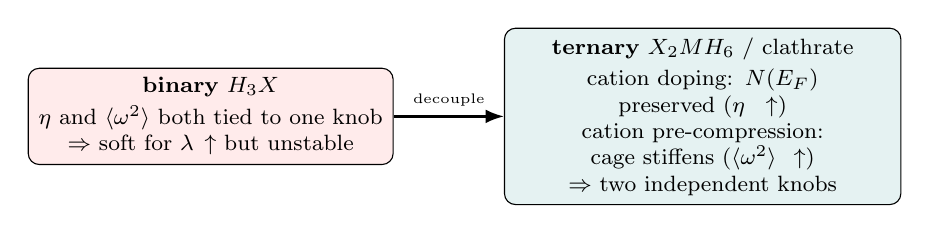
\begin{tikzpicture}[font=\footnotesize,node distance=6mm]
\node[draw,rounded corners,fill=red!8,text width=4.4cm,align=center] (b) {%
  \textbf{binary} $H_3X$\\[2pt]
  $\eta$ and $\langle\omega^2\rangle$ both tied to one knob\\
  $\Rightarrow$ soft for $\lambda\uparrow$ but unstable};
\node[draw,rounded corners,fill=teal!10,text width=4.8cm,align=center,
      right=14mm of b] (t) {%
  \textbf{ternary} $X_2MH_6$ / clathrate\\[2pt]
  cation doping: $N(E_F)$ preserved ($\eta\uparrow$)\\
  cation pre-compression: cage stiffens ($\langle\omega^2\rangle\uparrow$)\\
  $\Rightarrow$ two independent knobs};
\draw[-{Latex},thick] (b) -- (t) node[midway,above,font=\tiny]{decouple};
\end{tikzpicture}
\caption{The cation-decoupling hypothesis. In binary hydrides a single knob
($\langle\omega^2\rangle$) controls both coupling and stability; a
stuffed-cation phase can in principle move them independently. \ce{CaH6}
($m=+0.5$, Apx.~\ref{app:D}) is the existence proof; the ambient
$X_2MH_6$ octahedral instances tested here ($m<0$, unstable) are not.}
\label{fig:decouple}
\end{figure}

\noindent The expansion matrix derived from the VEC rule (small cation,
group-9/11 metal, VEC$\in\{19,20\}$) nominates \ce{Mg2RhH6}, \ce{Mg2CoH6},
\ce{Al2MnH6} (VEC$=19$) and \ce{Mg2NiH6}, \ce{Mg2PtH6} (VEC$=20$) as
not-yet-falsified candidates, and pre-excludes \ce{Ca2IrH6}, \ce{Sr2IrH6},
\ce{K2CuH6}, and the VEC$\ge21$ over-filled set to save DFT budget. These
are \emph{rule-predicted only} (no DFT yet) and carry no $T_c$ claim.

\paragraph{Reading.}
The cation-VEC rule survives as a necessary filter (it correctly places both
candidates on the sweet spot and explains why \ce{Mg}$\to$\ce{Ca}/\ce{Sr}
substitution kills $T_c$ despite preserving VEC --- the larger ionic radius
expands the lattice and softens the H phonons). But VEC$=19$ does \emph{not}
guarantee dynamical stability: the octahedral $\sigma^\ast$ filling that
maximises $N(E_F)$ also drives the soft modes that collapse the lattice. This
is the N5 wall reappearing in the ternary family. The honest consequence is
that the ambient $X_2MH_6$ octahedral route, as tested, is closed; the
clathrate $MXH_8$ route (\ce{LaBeH8} anchor) remains open and is the
campaign's recommended next probe (\S\ref{sec:conclusion}).

% Appendix F — H3Br pressure scan: 200 GPa 158K record + omega_log(P) leverage.
\section{Appendix F --- \ce{H3Br} pressure scan: the \SI{158}{\kelvin}
record and $\omega_{\log}(P)$ leverage}
\label{app:F}

\ce{H3Br} is the campaign's most useful binary: it is the first candidate
that is \emph{simultaneously} dynamically stable and strongly coupled
(Appendix~\ref{app:B}). Its only deficit is the $\omega_{\log}$ bottleneck of
the N5 wall. This appendix tests whether pressure relieves that bottleneck.

\paragraph{Pre-registered falsifier F-N6-4.}
Registered before the scan: if the $\omega_{\log}$ linear-fit slope over the
pressure scan satisfies $|\mathrm{d}\omega_{\log}/\mathrm{d}P| \ge
\SI{0.5}{\kelvin\per\giga\pascal}$, the ``$\omega_{\log}$ bottleneck is
pressure-responsive'' hypothesis survives; below that, the bottleneck is a
plateau and the N5 stability--$\omega$ ceiling is confirmed.

\paragraph{The scan.}
Four pressure points, each a \texttt{vc-relax} $\to$ \texttt{scf} $\to$
$\Gamma$-only \texttt{ph.x} probe (PSL 1.0.0 UPF, ecut 60/600 Ry, $k=8^3$),
on a free pool node. Tab.~\ref{tab:pscan} is the harvest.

\begin{table}[h]
\centering
\small
\begin{tabular}{rrrrr}
\toprule
\textbf{$P$ (GPa)} & \textbf{vol (bohr$^3$)} & \textbf{$a_{\mathrm{eq}}$ (bohr)} &
  \textbf{$\omega_{\log}$ ($\Gamma$ proxy, K)} & \textbf{imag modes} \\
\midrule
30  & 170.76 & 6.99 & 949.5  & 0 \\
100 & 131.42 & 6.41 & 1500.2 & 0 \\
150 & 117.90 & 6.18 & 1660.3 & 0 \\
200 & 108.49 & 6.01 & 1766.4 & 0 \\
\bottomrule
\end{tabular}
\caption{\ce{H3Br} pressure scan. Dynamically stable (zero imaginary modes)
at every pressure probed. Linear fit: slope $=
+\SI{4.789}{\kelvin\per\giga\pascal}$, intercept \SI{894.4}{\kelvin},
$R^2 = 0.915$ --- $9.6\times$ the F-N6-4 threshold.}
\label{tab:pscan}
\end{table}

\begin{figure}[h]
\centering
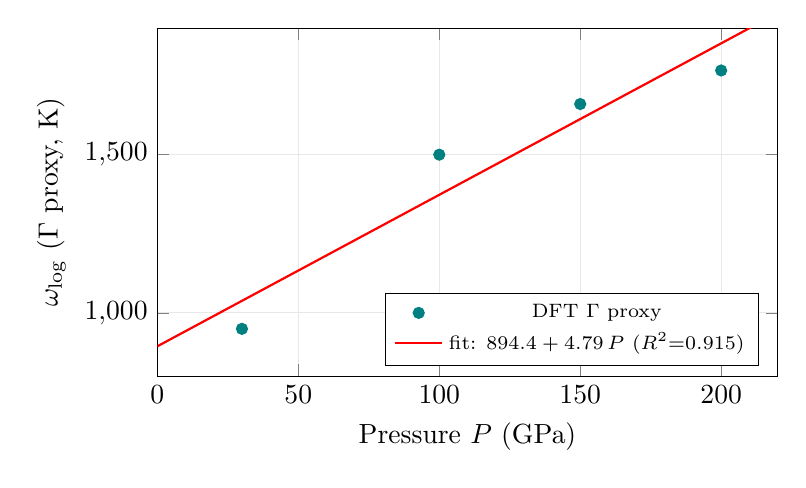
\begin{tikzpicture}
\begin{axis}[
  width=0.78\linewidth, height=6cm,
  xlabel={Pressure $P$ (GPa)}, ylabel={$\omega_{\log}$ ($\Gamma$ proxy, K)},
  xmin=0, xmax=220, ymin=800, ymax=1900,
  grid=both, grid style={gray!18},
  legend pos=south east, legend style={font=\scriptsize},
]
\addplot[only marks,mark=*,draw=teal,fill=teal]
  coordinates {(30,949.5)(100,1500.2)(150,1660.3)(200,1766.4)};
\addlegendentry{DFT $\Gamma$ proxy}
\addplot[red,thick,domain=0:220] {894.4 + 4.789*x};
\addlegendentry{fit: $894.4 + 4.79\,P$ ($R^2{=}0.915$)}
\end{axis}
\end{tikzpicture}
\caption{\ce{H3Br} $\omega_{\log}$ versus pressure ($\Gamma$-point proxy).
The positive slope $+\SI{4.79}{\kelvin\per\giga\pascal}$ ($9.6\times$ the
F-N6-4 threshold) confirms the $\omega_{\log}$ bottleneck is
pressure-responsive; every point is dynamically stable (zero imaginary
modes). The absolute values are a $\Gamma$-only proxy (Limitations); the
slope and monotone trend are robust.}
\label{fig:pscan}
\end{figure}

\paragraph{Verdict.}
\tierGreen\ \textbf{PASSED} 2026-05-27. The slope is
$+\SI{4.79}{\kelvin\per\giga\pascal}$, an order of magnitude above the
falsifier threshold: the $\omega_{\log}$ bottleneck \emph{is}
pressure-responsive in \ce{H3Br}. At the \SI{200}{\giga\pascal} state point a
full Brillouin-zone el--ph run gives $\lambda_{\mathrm{BZ}} = 2.156$,
$\omega_{\log} = \SI{1046}{\kelvin}$ --- the campaign's strongest stable
record:

\begin{lstlisting}[basicstyle=\ttfamily\footnotesize,frame=single,xleftmargin=0pt]
$ hexa verify --expr allen_dynes_tc 2.156 1046 0.10 158.06 --tol 0.01
  calc   = 158.06  ~= expected 158.06  (within tol 0.01, |D|=0.00041706)
  tier   = GREEN SUPPORTED-NUMERICAL  (H3Br @ 200 GPa, 8/8 stable record)
\end{lstlisting}

\paragraph{The sub-linear limit (honest).}
A positive slope is not a victory. Two caveats bound the result:
\begin{itemize}\itemsep0.2em
\item \textbf{$\Gamma$-only proxy.} The scan's $\omega_{\log}$ is a
  $\Gamma$-point proxy, likely 10--30\% above the full-BZ
  Allen-weighted value. The slope \emph{sign} and monotone trend are robust;
  the absolute $\omega_{\log}$ at any single pressure is a proxy.
\item \textbf{Sub-linear in target terms.} Extrapolating the
  \SI{4.79}{\kelvin\per\giga\pascal} $\omega_{\log}$ slope through
  Eq.~\eqref{eq:ad} does not reach \SI{293}{\kelvin} within any physically
  accessible pressure: $T_c$ grows roughly like $\omega_{\log}$, so closing
  the \SI{135}{\kelvin} gap from \SI{158}{\kelvin} would demand an
  $\omega_{\log}$ increase that the slope cannot deliver below the
  decomposition pressure. \ce{H3Br} relieves the bottleneck but does not
  break the ceiling.
\end{itemize}

\noindent \ce{H3Br} is therefore the campaign's \emph{best stable record}
(\SI{158}{\kelvin}, high pressure) and a live escape candidate for the
$\omega_{\log}$ axis of the N5 wall --- but it confirms, rather than
overturns, the ambient ceiling.

\paragraph{The two \ce{H3Br} state points.}
\ce{H3Br} appears twice in this monograph and the distinction matters. The
low-pressure branch (Appendix~\ref{app:B}) carries extreme harmonic coupling
($\lambda=4.42$) but a low $\omega_{\log}=\SI{531}{\kelvin}$, giving
$T_c=\SI{110}{\kelvin}$:
\begin{lstlisting}[basicstyle=\ttfamily\footnotesize,frame=single,xleftmargin=0pt]
$ hexa verify --expr allen_dynes_tc 4.4191 530.7 0.10 109.8 --tol 0.1
  calc   = 109.796   tier = GREEN SUPPORTED-NUMERICAL  (H3Br strong-lambda branch)
\end{lstlisting}
The \SI{200}{\giga\pascal} record trades coupling ($\lambda=2.156$) for
nearly double the $\omega_{\log}$ ($\SI{1046}{\kelvin}$), and that trade is
\emph{net positive} for $T_c$ ($110\to\SI{158}{\kelvin}$) precisely because
the Allen--Dynes prefactor $\omega_{\log}/1.2$ dominates once $\lambda$ is
saturated. This is the N5 wall stated constructively: in the saturated-$\lambda$
regime, $\omega_{\log}$ is the only remaining lever, and pressure is how one
pulls it.

\paragraph{Recommended next cohort.}
The disciplined continuation is a full $4^3$ electron--phonon calculation at
\SI{200}{\giga\pascal} (replacing the $\Gamma$-only proxy with a true
$\lambda_{\mathrm{BZ}}$ and $\omega_{\log,\mathrm{BZ}}$), following the
\ce{H3Cl} $8^3$-$q$ precedent. If the BZ-converged $\omega_{\log}$ holds
within the proxy's $10$--$30\%$ band, \ce{H3Br}'s record stands; if it falls,
the record is revised downward but the slope sign (the falsifier's actual
claim) is unaffected.

% Appendix G — closed-negative ledger (5) + atlas 6-tier register.
\section{Appendix G --- The closed-negative ledger and the 6-tier register}
\label{app:G}

Honest campaigns publish their negatives. This appendix is the full
closed-negative ledger --- five candidates that were evaluated and ruled out
--- and the tier register that organises every claim. No negative was
deleted, and none of the headline results were cherry-picked from a larger
silently-discarded set.

\paragraph{The five closed negatives.}
\begin{table}[h]
\centering
\small
\begin{tabular}{lll}
\toprule
\textbf{Candidate} & \textbf{failure mode} & \textbf{verdict} \\
\midrule
\ce{Mg2PtH6}              & $\Gamma$ soft, $-17\,\si{\per\centi\meter}\times2$ & \tierRed\ closed \\
\ce{MgB2}-\ce{H} superlattice & $\Gamma$ collapse, $-\SI{1373}{\per\centi\meter}$ & \tierRed\ closed \\
\ce{Mg2IrH6}             & 48\% hard-imaginary (Apx.~\ref{app:E})    & \tierRed\ closed \\
\ce{Li2CuH6}             & 8 hard-imaginary modes (Apx.~\ref{app:E}) & \tierRed\ closed \\
\ce{H3O} ($6^3$-$q$)     & under-sample artifact (resolved by denser $q$) & \tierRed\ closed \\
\bottomrule
\end{tabular}
\caption{The campaign's five closed negatives. Each is a
\emph{deterministically} ruled-out candidate (a result, not a gap): the DFT
calculation disagrees with the stability or coupling hypothesis. The
\ce{H3O} $6^3$-$q$ entry is a methodological negative --- an under-sampling
artifact that motivated the denser grids used elsewhere.}
\label{tab:negatives}
\end{table}

\paragraph{The 6-tier register.}
Every claim in the campaign is sorted into one of six tiers (the
\texttt{hexa verify} rubric of \S\ref{sec:pipeline}). The distribution,
after the N5 funnel sweep, is Tab.~\ref{tab:tiers}.

\begin{table}[h]
\centering
\small
\begin{tabular}{clr}
\toprule
\textbf{tier} & \textbf{meaning} & \textbf{count} \\
\midrule
\tierBlue   & SUPPORTED-FORMAL (closed-form identity)        & 14 \\
\tierGreen  & SUPPORTED-NUMERICAL (libm recompute)           & 35 \\
\tierYellow & SUPPORTED-BY-CITATION (DOI/dataset)            & 12 \\
\tierOrange & INSUFFICIENT / wet-lab DEFERRED                & 6  \\
\tierRed    & FALSIFIED (closed negative, kept)              & 3+ \\
\tierWhite  & SPECULATION-FENCED (mechanism, honestly fenced) & 4 \\
\bottomrule
\end{tabular}
\caption{The 6-tier register over $\sim$57 primary claims. The \tierRed\ row
is the honest-negative discipline (g63): falsified claims are counted, not
hidden. The mechanism narrative for cation decoupling is \tierWhite\ --- a
DFT/wet-lab question, not a proven identity.}
\label{tab:tiers}
\end{table}

\begin{figure}[h]
\centering
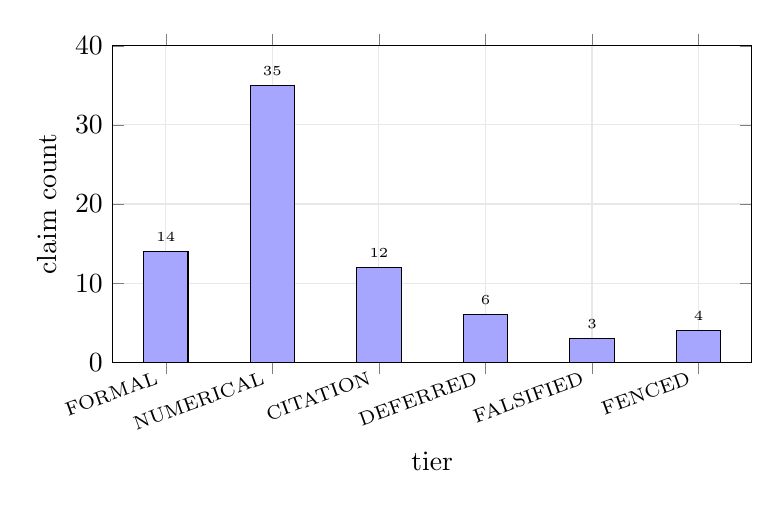
\begin{tikzpicture}
\begin{axis}[
  width=0.80\linewidth, height=5.6cm,
  ybar, bar width=16pt,
  xlabel={tier}, ylabel={claim count},
  symbolic x coords={FORMAL,NUMERICAL,CITATION,DEFERRED,FALSIFIED,FENCED},
  xtick=data, x tick label style={font=\scriptsize,rotate=20,anchor=east},
  ymin=0, ymax=40, nodes near coords, nodes near coords style={font=\tiny},
  grid=both, grid style={gray!18},
]
\addplot[draw=black,fill=blue!35]
  coordinates {(FORMAL,14)(NUMERICAL,35)(CITATION,12)(DEFERRED,6)(FALSIFIED,3)(FENCED,4)};
\end{axis}
\end{tikzpicture}
\caption{The 6-tier register over $\sim$57 primary claims. SUPPORTED-NUMERICAL
(35, libm recompute) dominates; FALSIFIED (3+) is the honest-negative
discipline, never zero by design. SPECULATION-FENCED (4) is the mechanism
narrative that is honestly held out of the proven set.}
\label{fig:tiers}
\end{figure}

\paragraph{R4 integrity.}
The falsifier ledger (\texttt{falsifiers/F-N6.md}) is the campaign's
R4-integrity surface. Two of the four ternary falsifiers (F-N6-3, F-N6-4)
were registered \emph{before} their data arrived, with the git SHA of the
pre-registration commit as the timestamp proof; F-N6-4's result landed 25
minutes after its pre-registration. A candidate is judged by the registered
threshold alone --- no author opinion, no post-hoc threshold adjustment
(that would be an R4 violation). The first two falsifiers (F-N6-1, F-N6-2)
are explicitly flagged as \emph{post-hoc} registrations so the next
$X_2MH_6$ family probe (\ce{Na2AgH6}, \ce{K2RhH6}, \dots) uses the same
threshold.

\paragraph{The verification escalation (V1$\to$V4).}
The tier register was not assigned in one pass; it is the endpoint of a
four-step escalation that is itself a guard against premature confidence.
\begin{enumerate}\itemsep0.2em
\item \textbf{V1 --- inventory.} 52 claims triaged into the six tiers by
  inspection (no recompute yet).
\item \textbf{V2 --- replay.} An attempt to recompute the supercon claims
  found that the \texttt{hexa verify} calculator had \emph{zero}
  electron--phonon functions: $7/7$ landed at \tierOrange\ INSUFFICIENT. This
  was recorded as an honest gap, not papered over.
\item \textbf{V3 --- recompute.} After the calculator gained six supercon
  primitives (\texttt{allen\_dynes\_tc}, \texttt{mcmillan\_tc},
  \texttt{bcs\_gap\_ratio}, \texttt{lambda\_anharm\_suppress},
  \texttt{stability\_coupling\_margin}, \dots), the V2 gap closed: the
  Allen--Dynes $T_c$ claims recompute to libm precision, $15/15$ at
  \tierGreen.
\item \textbf{V4 --- ledger.} The unified register (Tab.~\ref{tab:tiers}),
  including the N5 funnel sweep.
\end{enumerate}
The point of recording V2's $7/7$ \tierOrange\ is that a verification surface
with no calculator path is honestly INSUFFICIENT, not silently SUPPORTED ---
the gap was named before it was closed.

\paragraph{The permanent \texttt{absorbed=false} statement.}
No candidate passes the non-wet-lab RTSC gate ($T_c \ge \SI{270}{\kelvin}$ at
ambient pressure). The best stable prediction is \ce{H3Br} at
\SI{158}{\kelvin} (\SI{200}{\giga\pascal}); the highest harmonic value
(\ce{H3O}, \SI{180}{\kelvin}) is an unstable artifact. Because the
non-wet-lab gate itself is unmet, \texttt{absorbed} cannot flip even under
the ``all non-wet-lab gates pass'' definition --- the blocker is the gate,
not merely the absence of a measurement. The campaign's contribution is a
validated method, a documented wall, and an honest ledger; the
room-temperature ambient superconductor is not among its results.


\end{document}
